\documentclass[12pt,a4paper]{article}

\usepackage[margin=1in]{geometry}
\usepackage{setspace}
\usepackage{amsmath,amssymb}
\usepackage{graphicx}
\usepackage{booktabs}
\usepackage{float}
\usepackage{caption}
\usepackage{hyperref}
\usepackage{xcolor}
\usepackage{listings}
\usepackage{fancyhdr}

\onehalfspacing
\setlength{\parskip}{0.4em}
\setlength{\parindent}{2em}
\setlength{\headheight}{15pt}

\hypersetup{
  colorlinks=true,
  linkcolor=blue!60!black,
  urlcolor=blue!60!black
}

\lstdefinestyle{matlabstyle}{
  language=Matlab,
  basicstyle=\ttfamily\small,
  keywordstyle=\color{blue!70!black},
  commentstyle=\color{green!40!black},
  stringstyle=\color{orange!70!black},
  numbers=left,
  numberstyle=\tiny\color{gray},
  stepnumber=1,
  numbersep=8pt,
  frame=single,
  breaklines=true,
  showstringspaces=false
}

\pagestyle{fancy}
\fancyhf{}
\lhead{ICE4405P DSP Lab 1}
\rhead{Weile Mo\ \ \ 523260910022}
\cfoot{\thepage}

\title{\textbf{ICE4405P Digital Signal Processing\\Lab 1 Report}\\[0.6em]
\large Convolution, DTFT, Z-Transform}
\author{Student Name: Weile Mo\\Student ID: 523260910022}
\date{2026-04-02}

\begin{document}

\maketitle
\thispagestyle{empty}
\newpage

\tableofcontents
\newpage

\section{Problem 1: Simulating a Recording Studio's Reverberation}

\subsection{Given}
$$
h[n] = \delta[n] + 0.5\delta[n-1] + 0.3\delta[n-2]
$$
$$
x[n] = [2,\ 4,\ 6,\ 4,\ 2,\ 0]
$$

\subsection{Method}
Compute the reverberated output using discrete-time convolution:
$$
y[n] = x[n] * h[n]
$$
MATLAB command:
\begin{lstlisting}[style=matlabstyle]
y = conv(x, h);
\end{lstlisting}

\subsection{Result}
$$
y[n] = [2,\ 5,\ 8.6,\ 8.2,\ 5.8,\ 2.2,\ 0.6,\ 0]
$$

\subsection{Figure}
\begin{figure}[H]
  \centering
  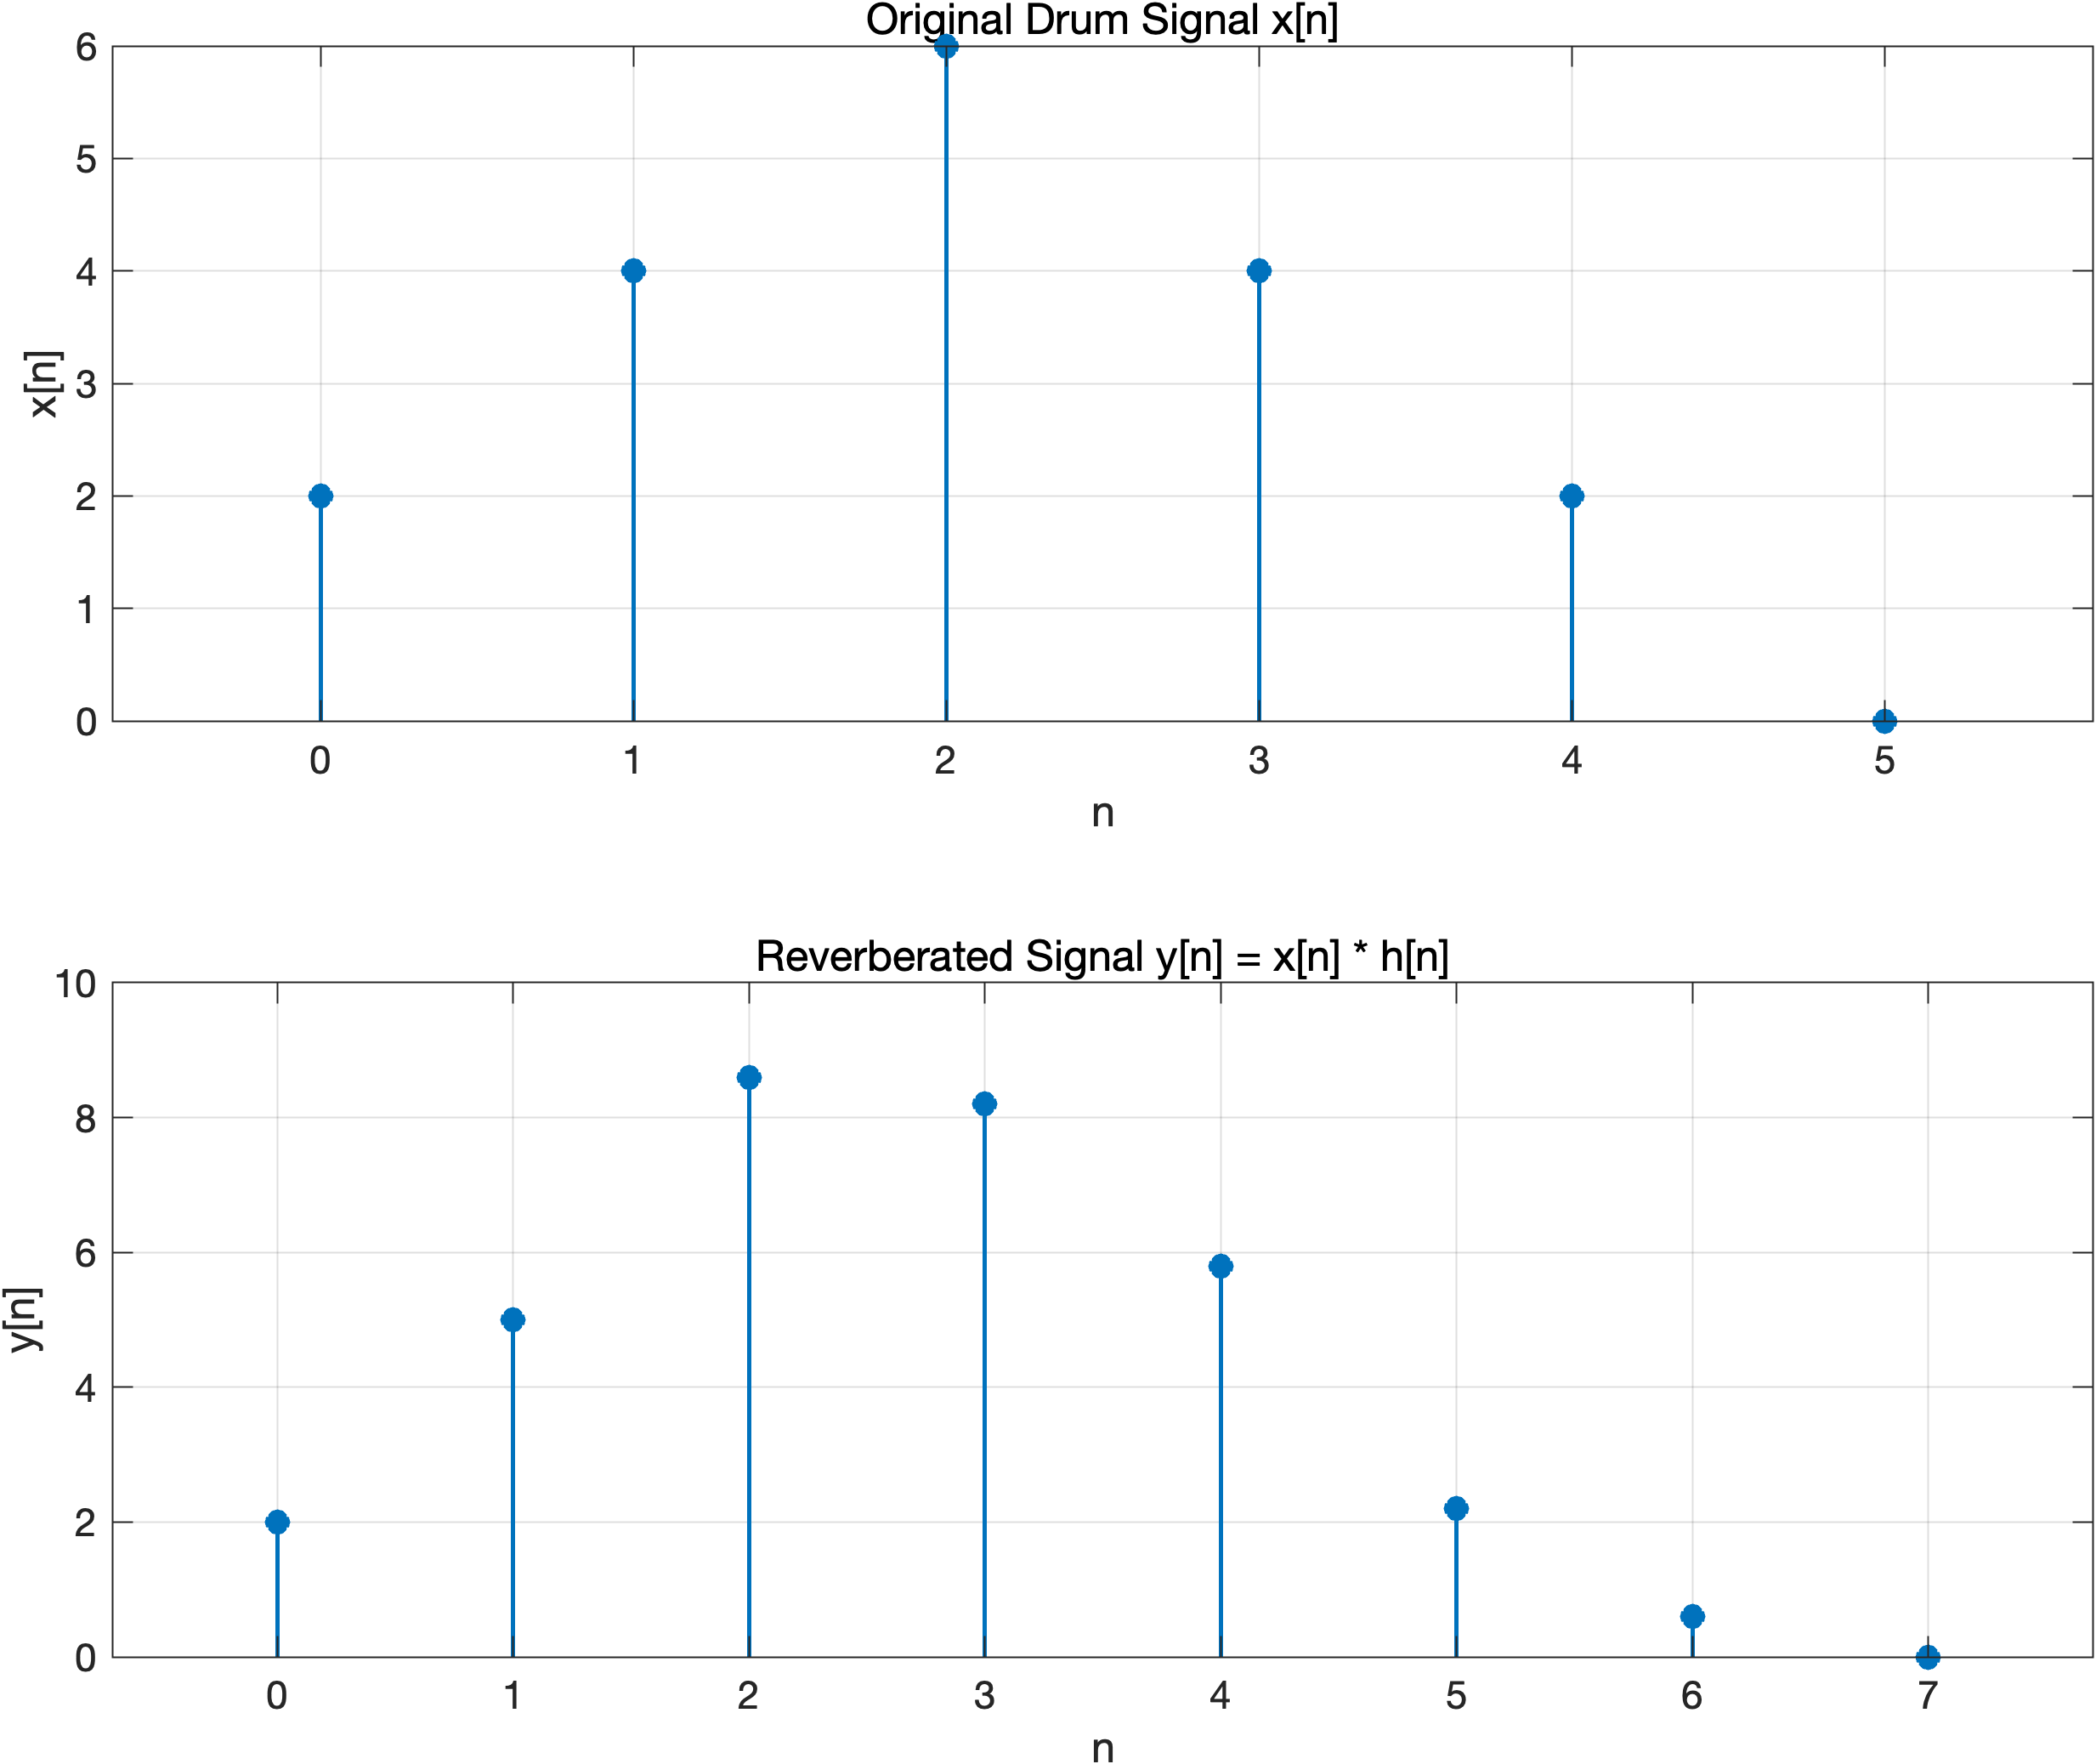
\includegraphics[width=0.9\textwidth]{Problem1.png}
  \caption{Problem 1: Original and reverberated signals}
\end{figure}

\subsection{Discussion}
The output sequence is longer than the original sequence and shows smoother decay, consistent with reverberation introduced by delayed and attenuated reflections.

\section{Problem 2: Simulating Echo in an Open Space}

\subsection{Given}
$$
x[n] = 0.8^n,\quad 0 \le n \le 10
$$
$$
h[n] = \delta[n] + 0.5\delta[n-1] + 0.3\delta[n-2]
$$

\subsection{Method}
Compute echoed signal:
$$
y[n] = x[n] * h[n]
$$
MATLAB command:
\begin{lstlisting}[style=matlabstyle]
n = 0:10;
x = 0.8.^n;
y = conv(x, h);
\end{lstlisting}

\subsection{Result}
First several samples:
$$
y[n] = [1,\ 1.3,\ 1.34,\ 1.072,\ 0.8576,\ \cdots]
$$

\subsection{Figure}
\begin{figure}[H]
  \centering
  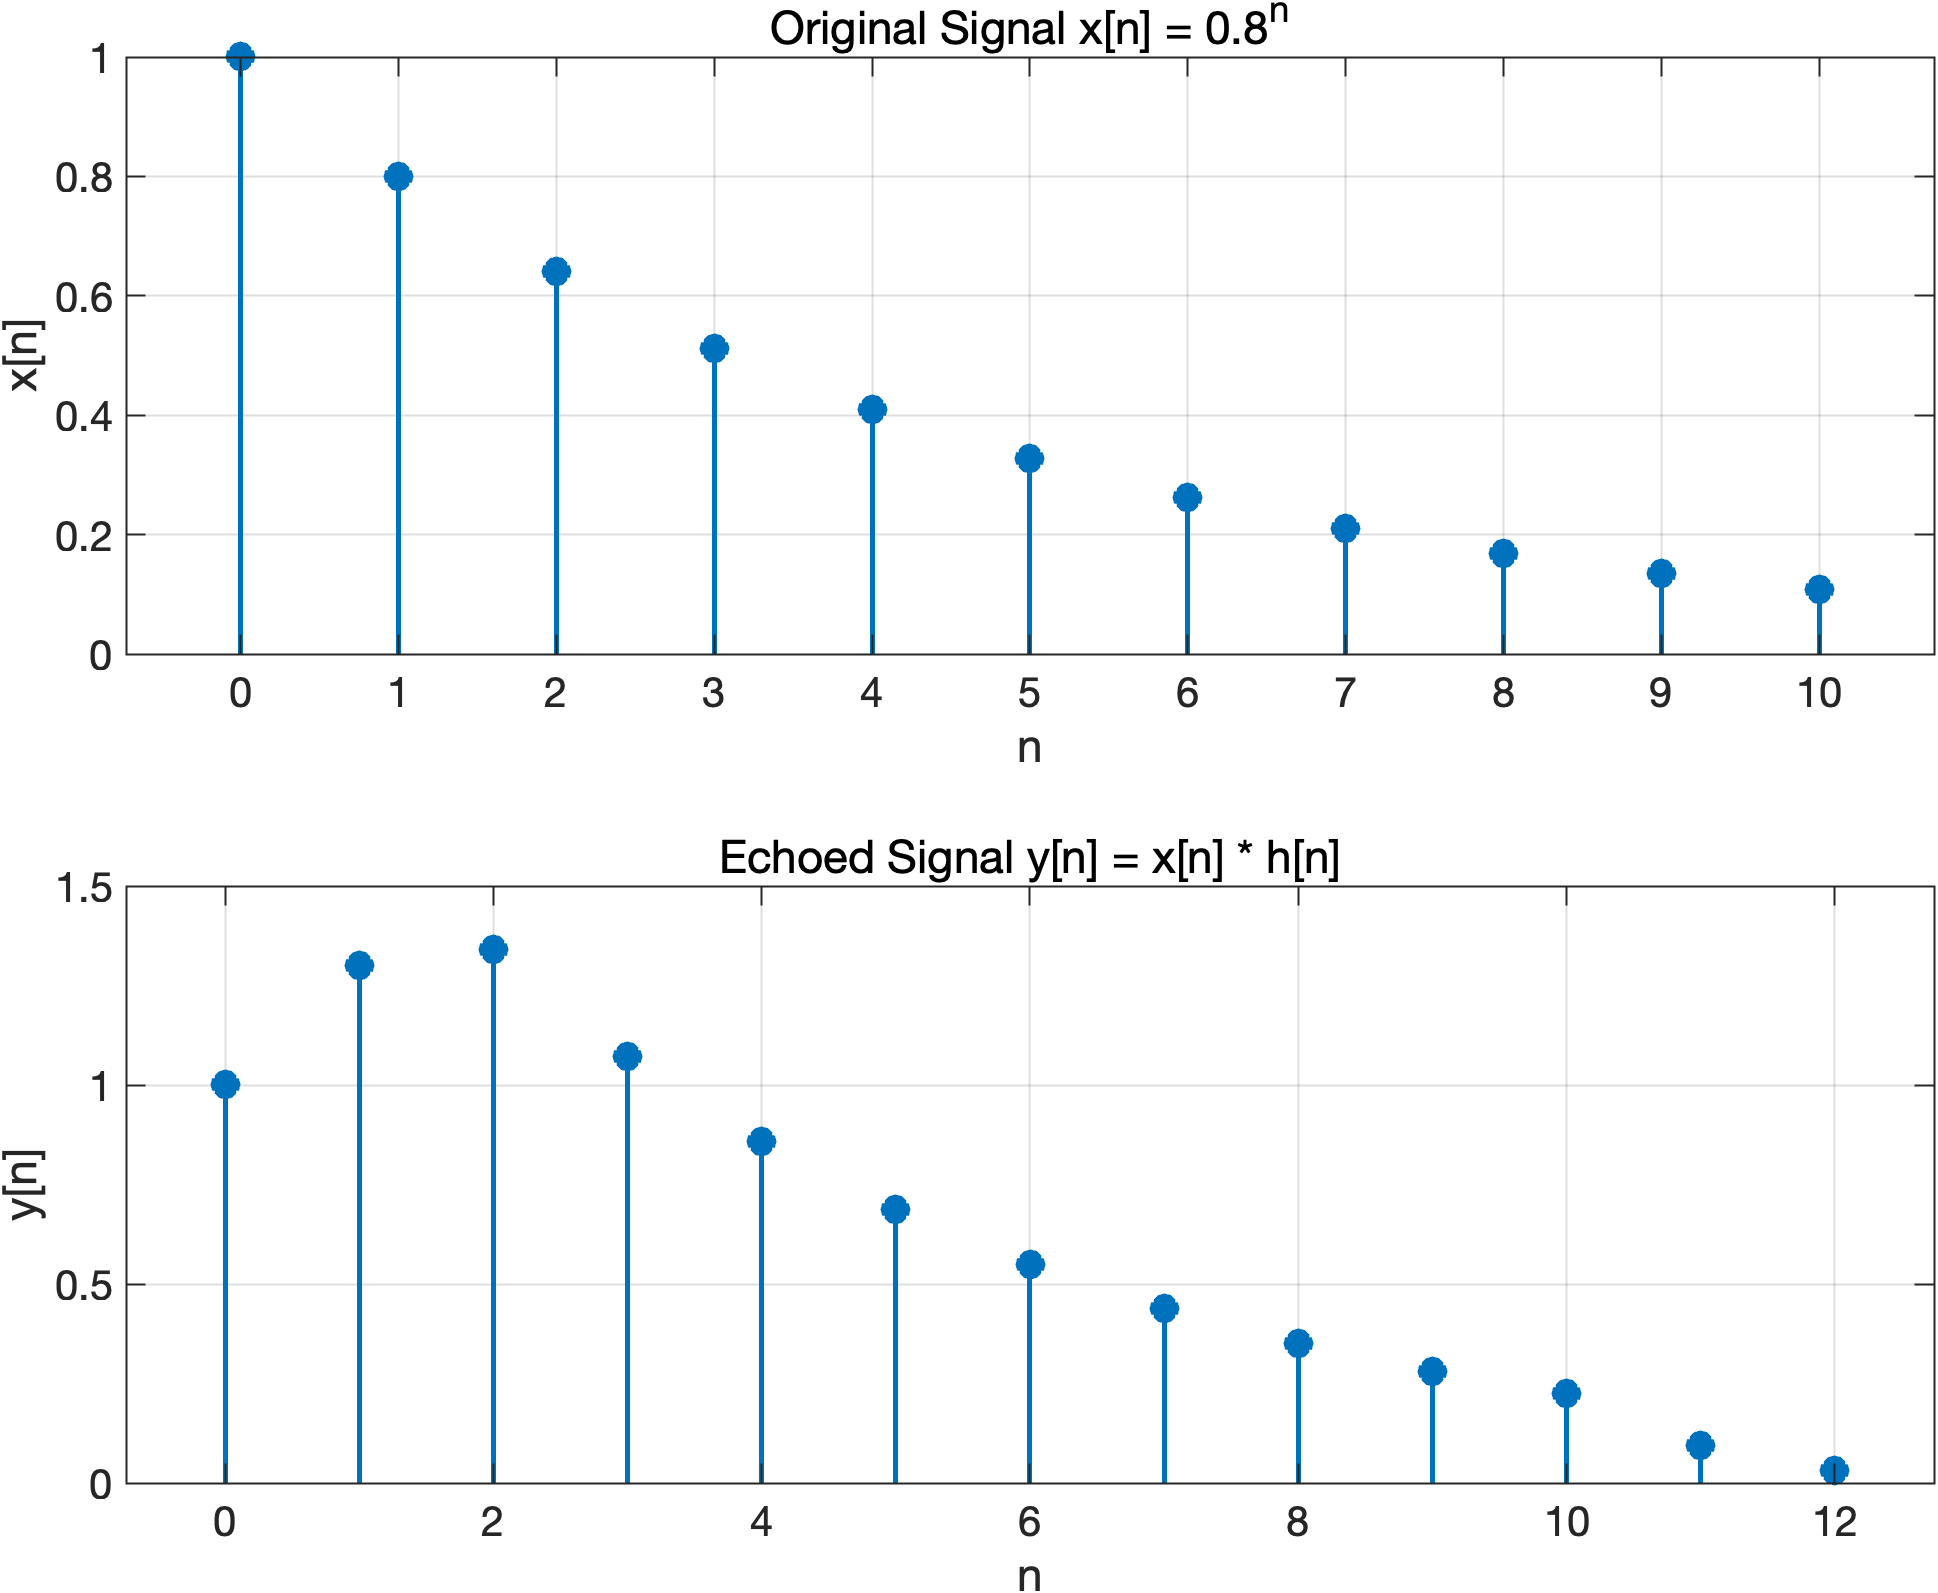
\includegraphics[width=0.9\textwidth]{Problem2.png}
  \caption{Problem 2: Original and echoed signals}
\end{figure}

\subsection{Discussion}
The echoed signal has larger early samples and a longer tail than the original decaying sequence, matching expected multi-path reflection behavior.

\section{Problem 3: Spectrum Analysis of a Speech Signal (DTFT)}

\subsection{Given}
$$
x[n] = 0.8^n,\quad 0 \le n \le 10
$$

\subsection{DTFT}
$$
X(\omega) = \sum_{n=-\infty}^{\infty}x[n]e^{-j\omega n}
$$
For this finite-length sequence:
$$
X(\omega) = \sum_{n=0}^{10}(0.8)^n e^{-j\omega n}
$$

\subsection{Method}
Numerically evaluate $X(\omega)$ over $\omega \in [-\pi,\pi]$, then plot:
$$
|X(\omega)|,\quad \angle X(\omega)
$$

\subsection{Figure}
\begin{figure}[H]
  \centering
  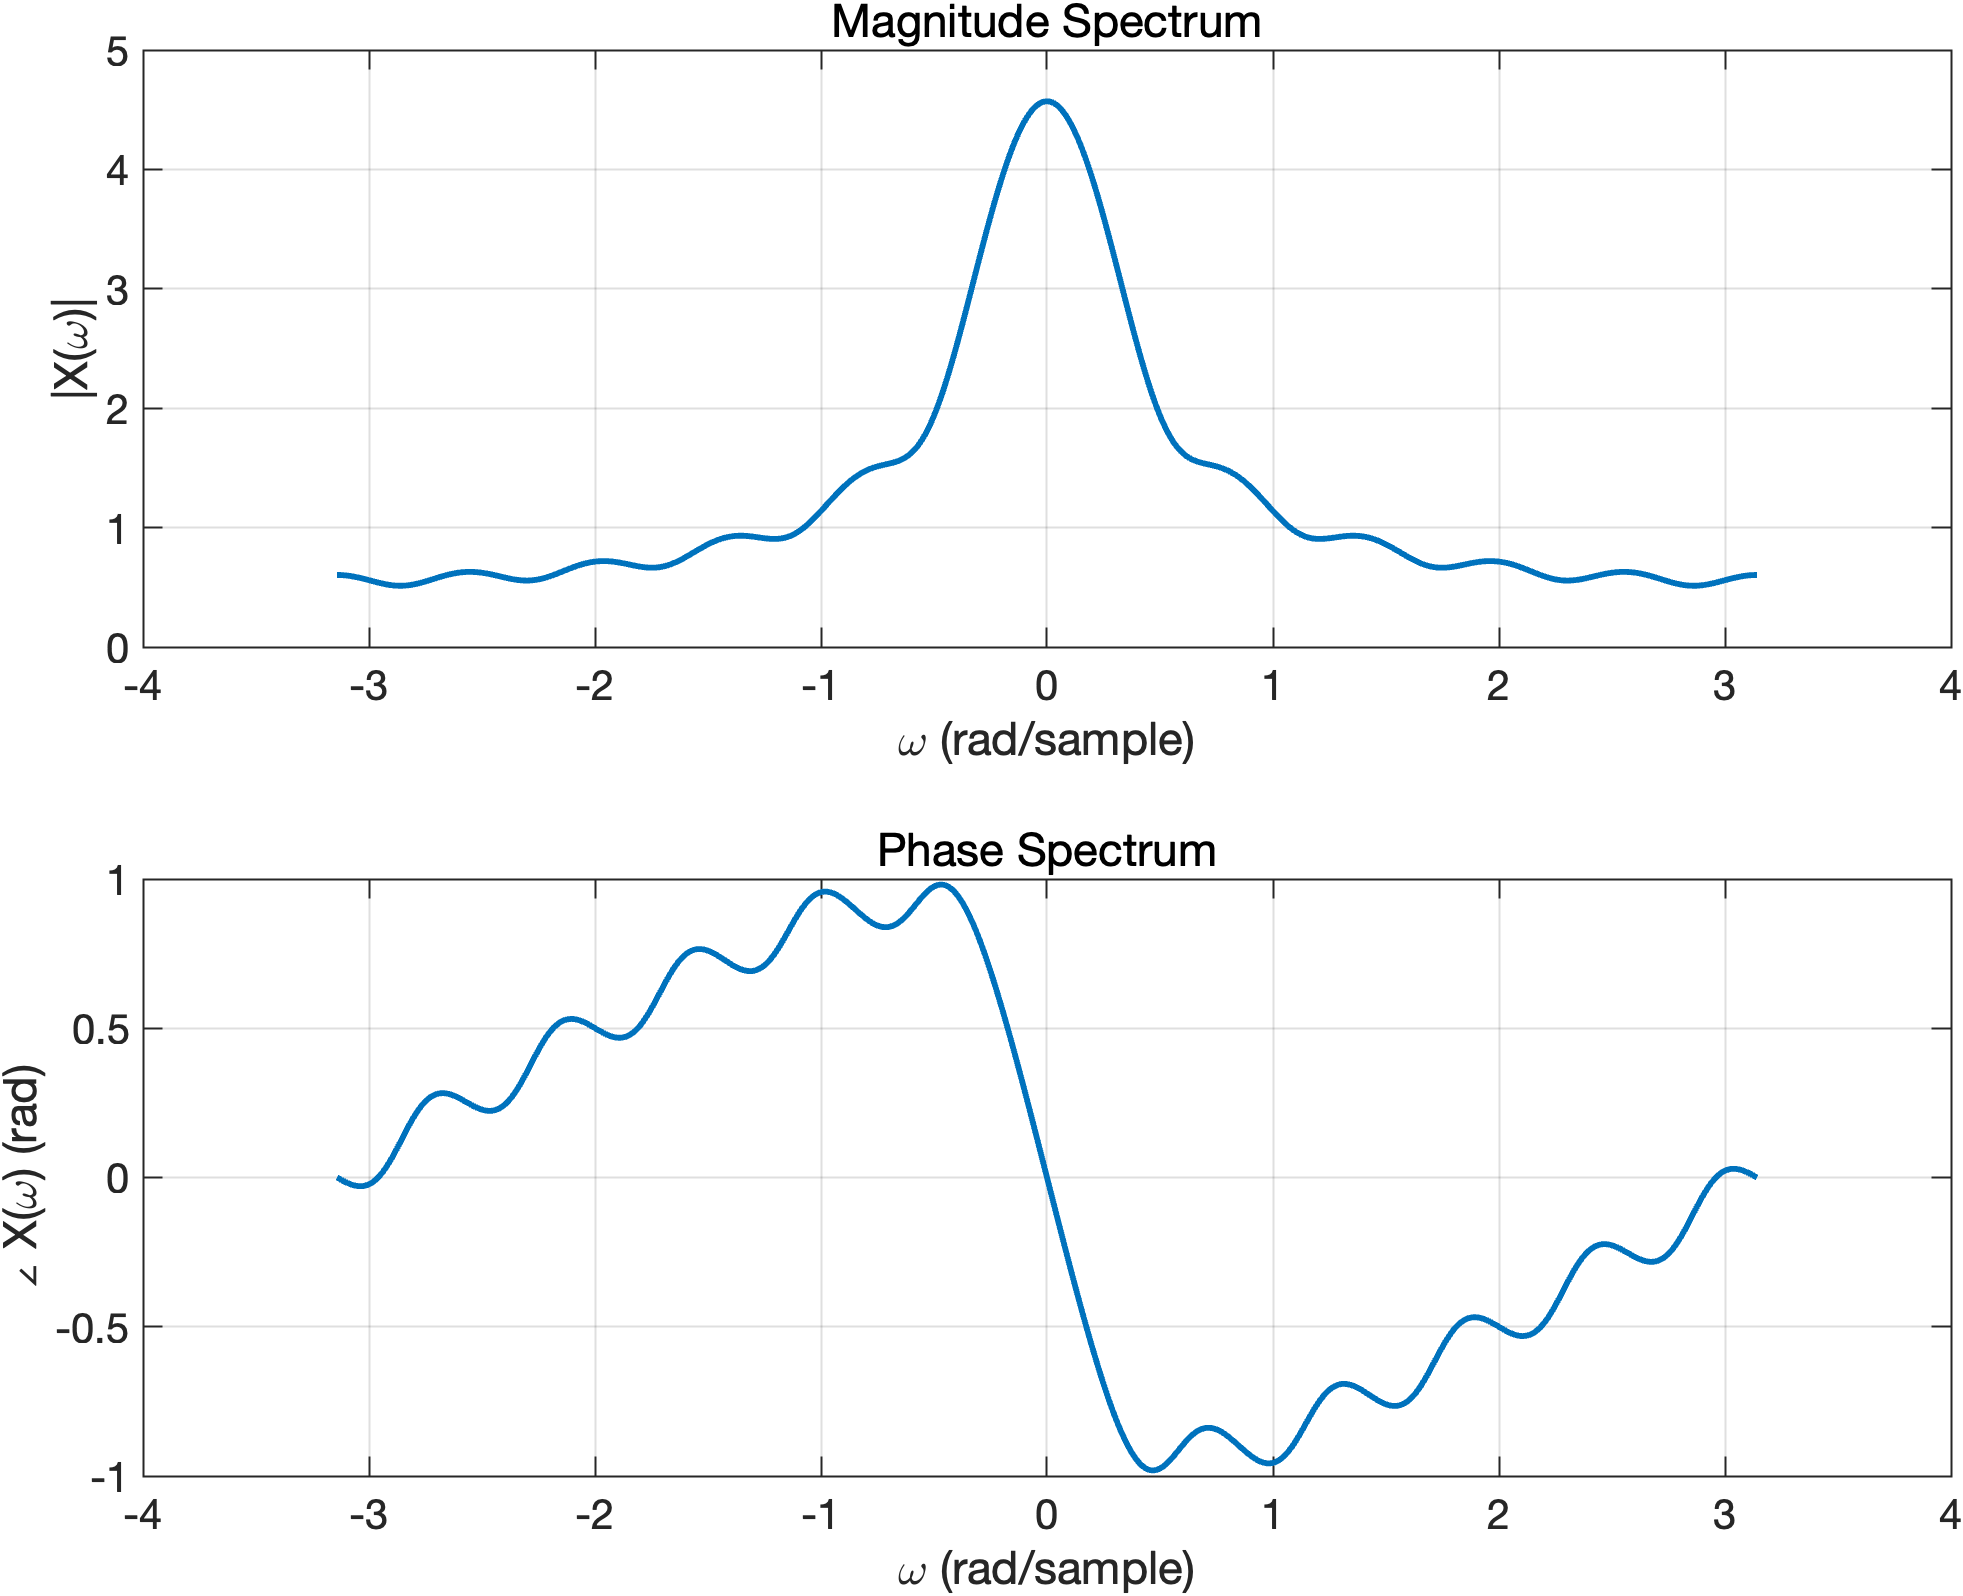
\includegraphics[width=0.9\textwidth]{Problem3.png}
  \caption{Problem 3: Magnitude and phase spectra of DTFT}
\end{figure}

\subsection{Discussion}
The magnitude is strongest near $\omega=0$, indicating that low-frequency components dominate this exponentially decaying sequence.

\section{Problem 4: High-Pass Filter for Speech Enhancement}

\subsection{Given}
$$
h[n] = (-0.5)^n u[n]
$$

\subsection{Z-Transform and ROC}
$$
H(z) = \sum_{n=0}^{\infty}(-0.5)^n z^{-n}
= \frac{1}{1+0.5z^{-1}}
$$
Pole location:
$$
z=-0.5
$$
Region of convergence:
$$
\mathrm{ROC}: |z|>0.5
$$

\subsection{Stability and Interpretation}
Since $|{-0.5}|<1$ and the ROC includes the unit circle, the filter is stable.
Also, from the frequency response:
$$
|H(e^{j\pi})| > |H(e^{j0})|
$$
it emphasizes higher frequencies, which is consistent with high-pass behavior and useful for suppressing low-frequency interference in speech enhancement.

\subsection{Figure}
\begin{figure}[H]
  \centering
  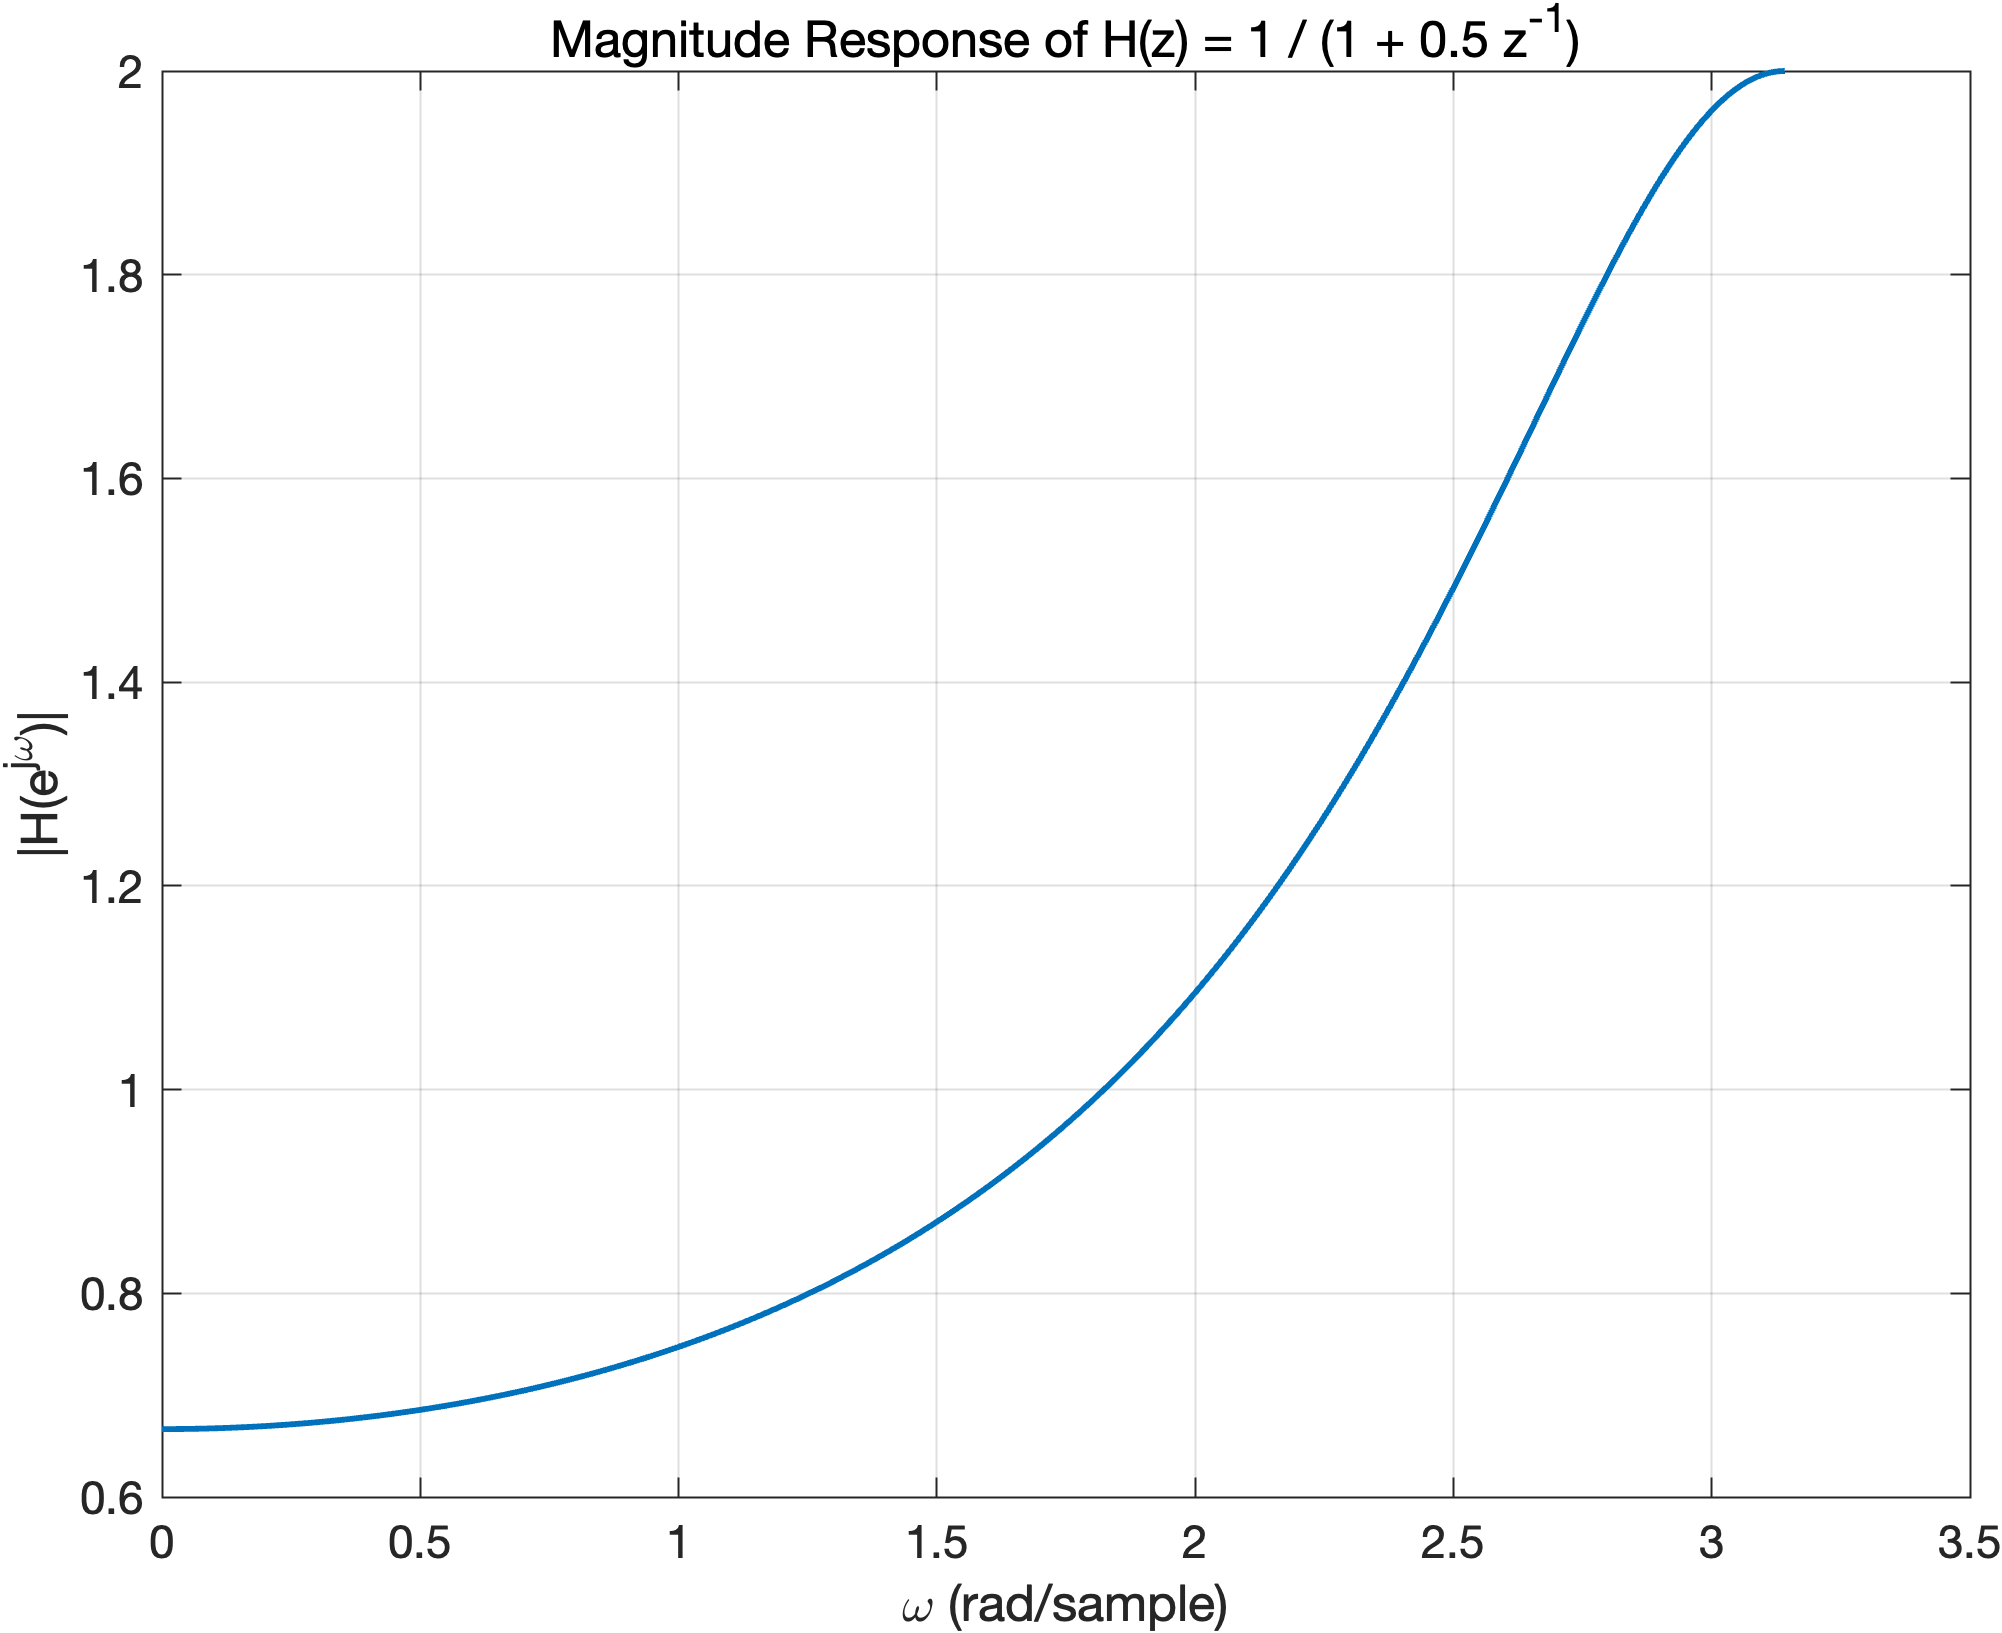
\includegraphics[width=0.9\textwidth]{Problem4.png}
  \caption{Problem 4: Magnitude response of high-pass filter}
\end{figure}

\section{Problem 5: Stability Analysis of a Low-Pass Filter}

\subsection{Given}
$$
h[n] = (0.7)^n u[n]
$$

\subsection{Z-Transform and ROC}
$$
H(z) = \sum_{n=0}^{\infty}(0.7)^n z^{-n}
= \frac{1}{1-0.7z^{-1}}
$$
Pole location:
$$
z=0.7
$$
Region of convergence:
$$
\mathrm{ROC}: |z|>0.7
$$

\subsection{Stability and Comparison}
Since $|0.7|<1$ and the unit circle is included in ROC, this filter is stable.
For this filter:
$$
|H(e^{j0})| > |H(e^{j\pi})|
$$
so it has low-pass behavior. Compared with Problem 4, Problem 5 is better for smoothing and low-frequency preservation, while Problem 4 is better for suppressing low-frequency components.

\subsection{Figure}
\begin{figure}[H]
  \centering
  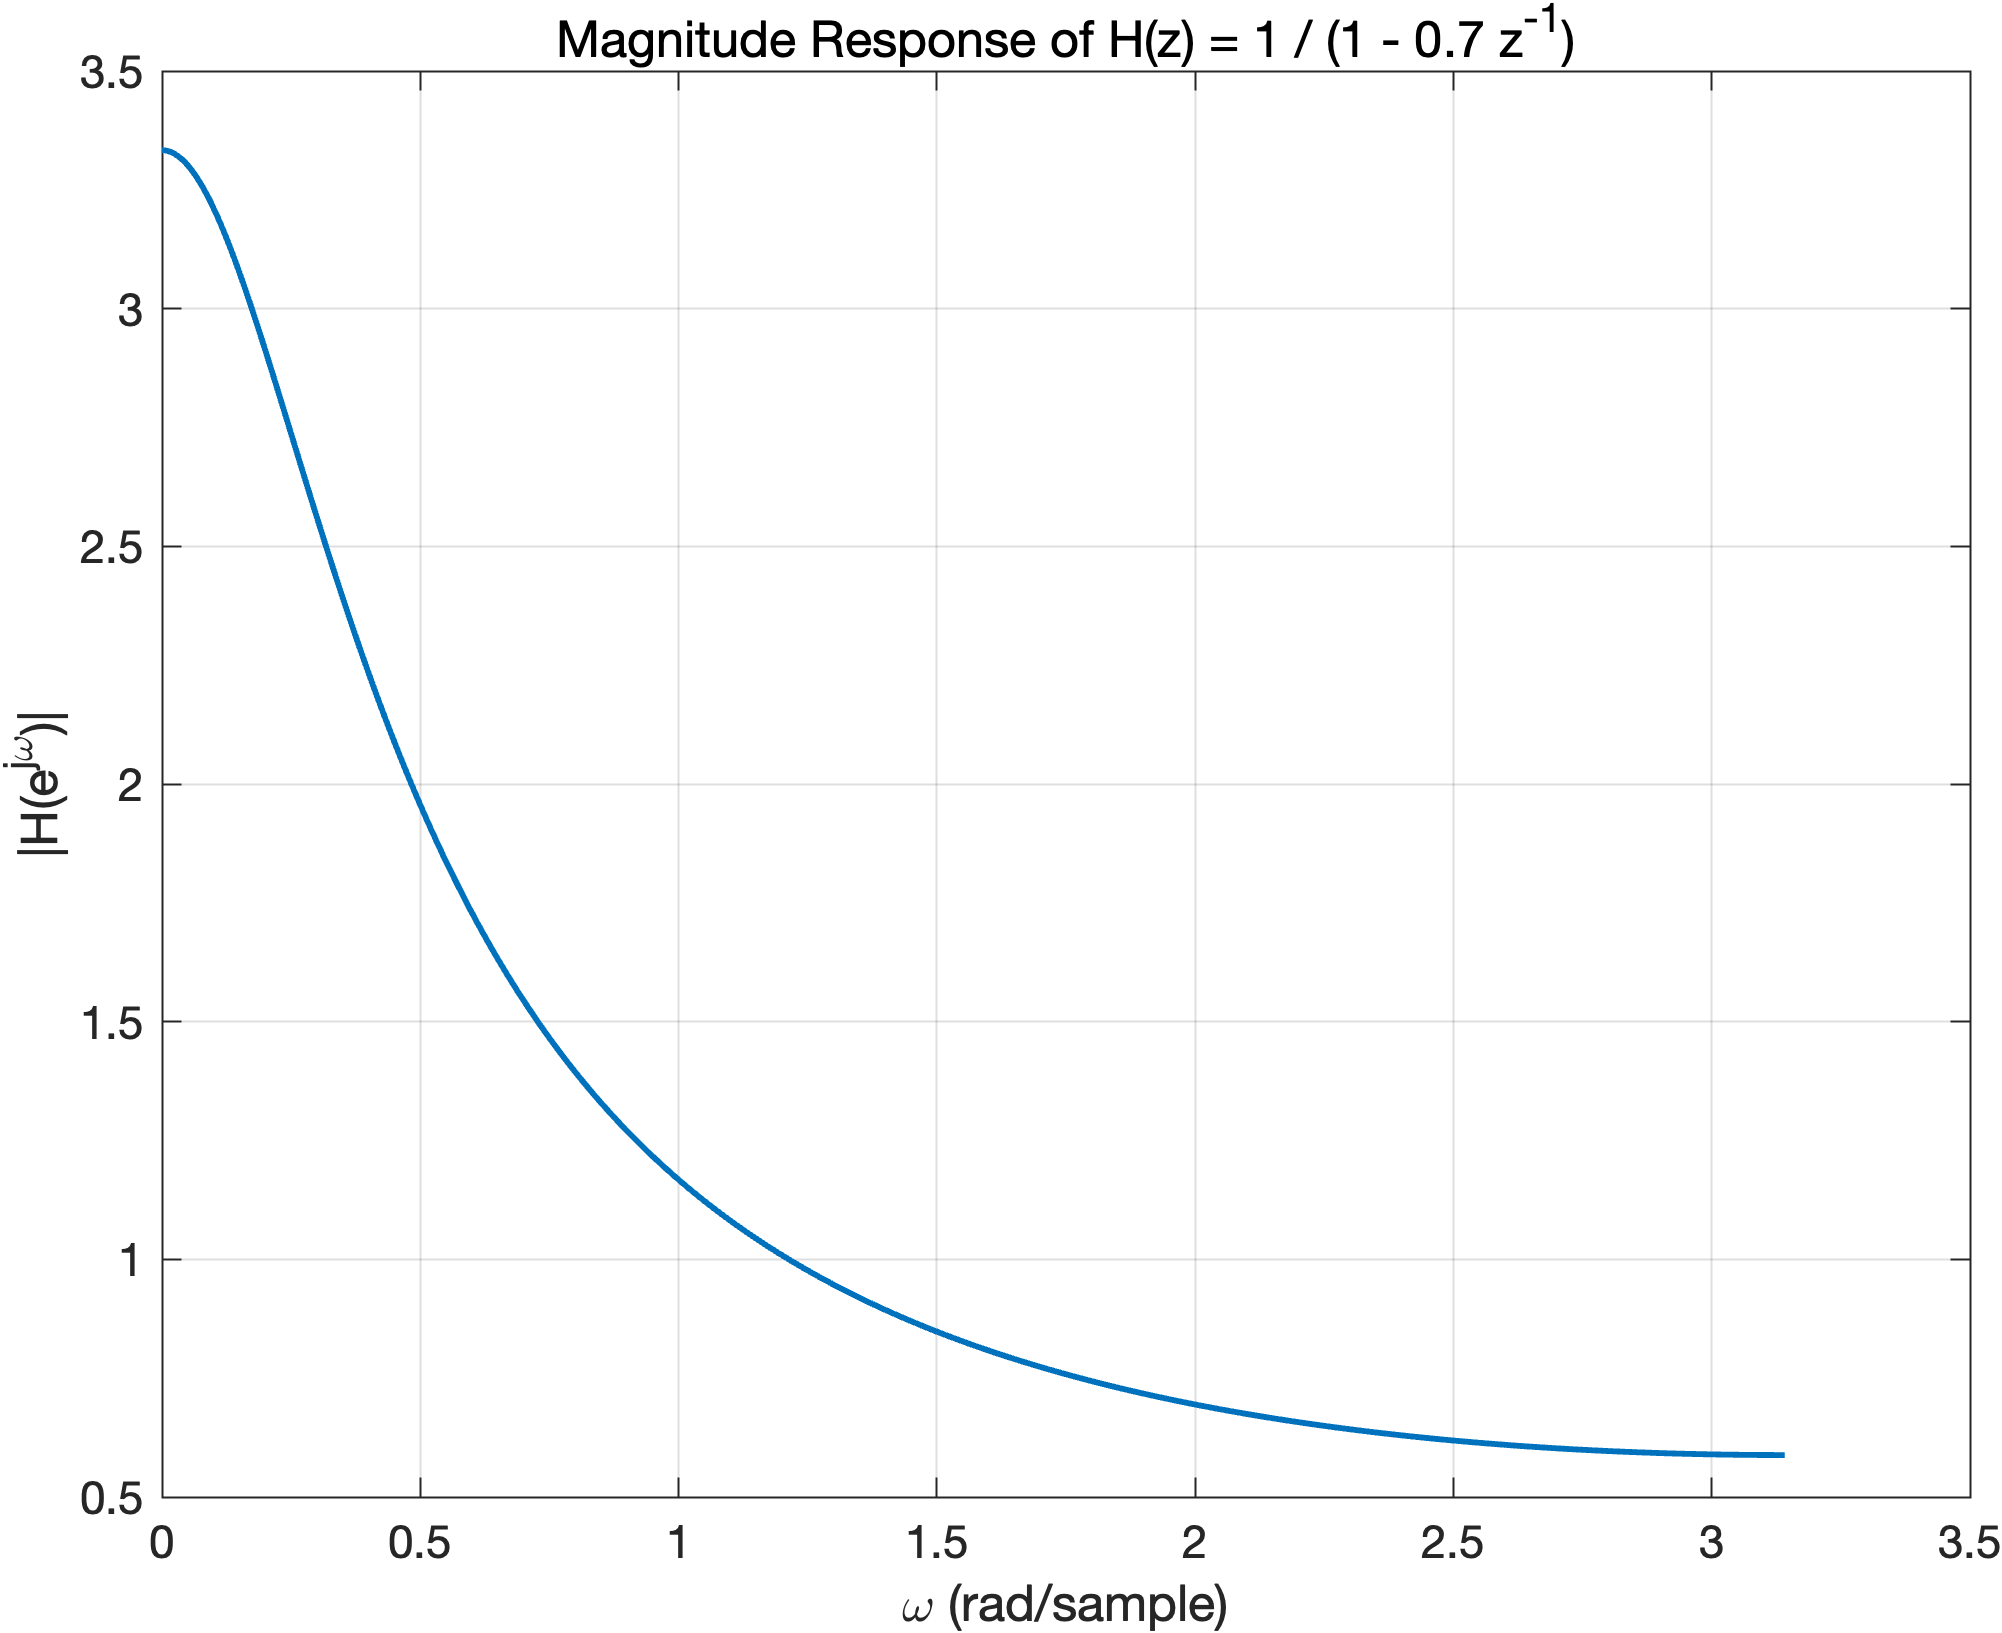
\includegraphics[width=0.9\textwidth]{Problem5.png}
  \caption{Problem 5: Magnitude response of low-pass filter}
\end{figure}

\section{Conclusion}
This lab verifies three core DSP tools:
\begin{enumerate}
  \item Convolution for time-domain system effects (reverberation/echo),
  \item DTFT for frequency-domain analysis,
  \item Z-transform for pole/ROC-based stability and filter interpretation.
\end{enumerate}
Both filters in this lab are stable but provide different frequency-selective behavior for speech processing tasks.

\end{document}
